\documentclass[onecolumn,12pt]{asme2ej}
\usepackage{epsfig}\usepackage{amsmath}\usepackage{amsfonts}
\usepackage{amssymb}\usepackage{graphicx}\pagenumbering{arabic}
\usepackage{verbatim}\usepackage[utf8]{inputenc}\usepackage[portuguese]{babel}
\providecommand{\keywords}[1]{\small\textbf{\textit{Keywords---}} #1}
\usepackage{comment}
\usepackage[backend=biber,style=numeric,sorting=none]{biblatex}
\usepackage{fancyhdr}\usepackage{pifont}
\usepackage{tikzsymbols}\usepackage{placeins}
\usepackage{rotating}
\pagestyle{fancy}\fancyhf{}\rfoot{Página \thepage}

\addbibresource{mybib.bib} \iffalse É neste arquivo que as referências ficam. \fi

\title{ Simulação de Investimentos por Classe de Ativos}

\author{Gustavo Foroutan Raposo \affiliation{PUCPR\\Ciência da Computação\\gustavo.raposo@pucpr.edu.br}}

\author{Gustavo Hammerschmidt\affiliation{PUCPR\\Ciência da Computação\\g.hammerschmidt@pucpr.edu.br}}

\author{João Felipe Schwab Teixeira Dos Santos \affiliation{PUCPR\\Ciência da Computação\\joao.schwab@pucpr.edu.br}}

\author{Matheus Willhelm Siqueira \affiliation{PUCPR\\Ciência da Computação\\matheus.siqueira@pucpr.edu.br}}

\author{Ricardo Naoki Tanji \affiliation{PUCPR\\Ciência da Computação\\ricardo.tanji@pucpr.edu.br}}


\begin{document}

\maketitle
\newpage
$\\ \\$
\begin{abstract} \iffalse To Do \fi
{\it 

Frequentemente, questiona-se a diferença entre investir em ativos com bons fundamentos e investir em ativos bem-falados ou que estão em foco pelo público geral. Fizemos uma simulação pautada em indicadores de mercado para classes de ativos com aplicação e controle do capital investido a cada trimestre. A equipe utilizou várias técnicas e indicadores. Para entender o movimento de mês em mês, utilizamos o comportamento das médias móveis, reversões majoritárias de tendência, saúde do mercado etc. Os resultados obtidos apontam que a classe de ativos apreciando de valor têm um impacto mais positivo aos ativos depreciando, e que especulá-los pode impactar diretamente no montante investidos caso não haja um bom planejamento.

}
\end{abstract}
\keywords{Investimentos, Classes, Simulação}

\newpage \tableofcontents \newpage

\section{Introdução} 

Constantemente, os investidores precisam reavaliar seus planos de investimentos. Muitas vezes, ativos considerados bons podem mudar sua classificação de risco. Mas não só isso: há, também, a distinção de investimentos em ativos de valor e ativos com potencial de precificação. Investir em ações pelo seu valor ou pelo seu preço? 

Às vezes, especular o preço de um ativo pode trazer bons ganhos para o portfólio, sem que a empresa tenha mesmo o valor a que está sendo negociada. Porém, há riscos nessa modalidade e muitos investidores procuram apenas ativos de valor - por mais que esses ativos já estejam bem caros.

Para resolver o problema dessa paridade, simulamos um ambiente com 10 ativos e retornos hipotéticos aleatoriamente, junto de índices e possíveis mudanças na perspectiva sobre os ativos para alocar o capital definido.

\section{Revisão Teórica e Contribuições}

Para simular este cenário de investimentos, a equipe utilizou várias técnicas e indicadores. Para entender o movimento de mês em mês, utilizamos o comportamento das médias móveis de 8 períodos e de 22 períodos para definir um bom momento de entrada ou saída de uma porcentagem de capital definida para cada classe de ativos definida\cite{artigo1} [Veja a seção metodologia]. Para evitar perdas em entradas e saídas recorrentes, utilizamos o indicador de reversão de tendência majoritária para os ativos\cite{artigo3}.

No que tange ao cenário global de investimentos, utilizamos o índice Bovespa\cite{artigo2} e o coeficiente BETA\cite{artigo6} para definir a saúde do mercado e o grau de risco atrelado ao ativo respectivamente. 

E, para evitar negociar empresas rentáveis com frequência, utilizamos a estimativa de dívida bruta em relação ao fluxo de caixa da empresa associada ao ativo\cite{artigo4}\cite{artigo5}. Esta relação índica se estamos vendendo um negócio que pode se valorizar muito com o tempo.


\section{Metodologia}


Para realizar a simulação, modelamos os fatores de decisão utilizando a aleatoriedade. 

\FloatBarrier
\begin{figure}[h]
    \centering
    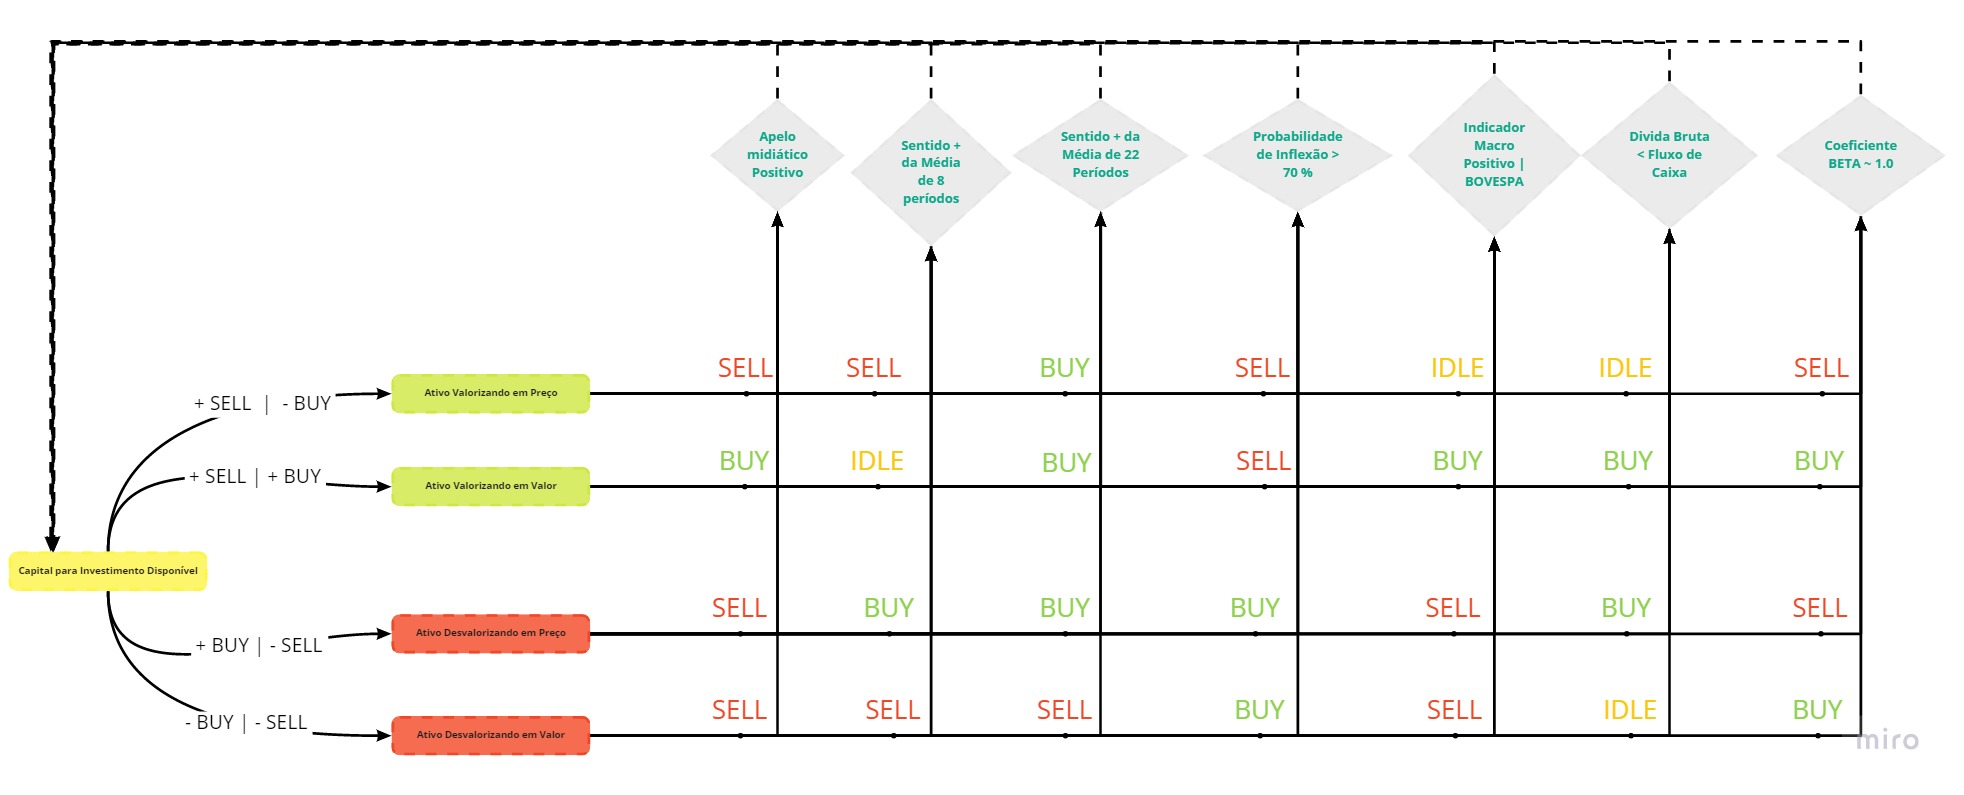
\includegraphics[width=15cm]{SIMUL/full.jpg}
    \caption{Grafo de Tomada de Decisão.}
    \label{fig:g1}
\end{figure}
\FloatBarrier

Perceba que definimos quatro tipos de ativos: aqueles que estão apreciando e possuem valor; aqueles que estão apreciando em preço e podem não ter um fundamento sólido e valor; aqueles que estão depreciando em preço e podem ter um fundamento sólido e valor; e aqueles que estão depreciando e não possuem valor.

\FloatBarrier
\begin{figure}[h]
    \centering
    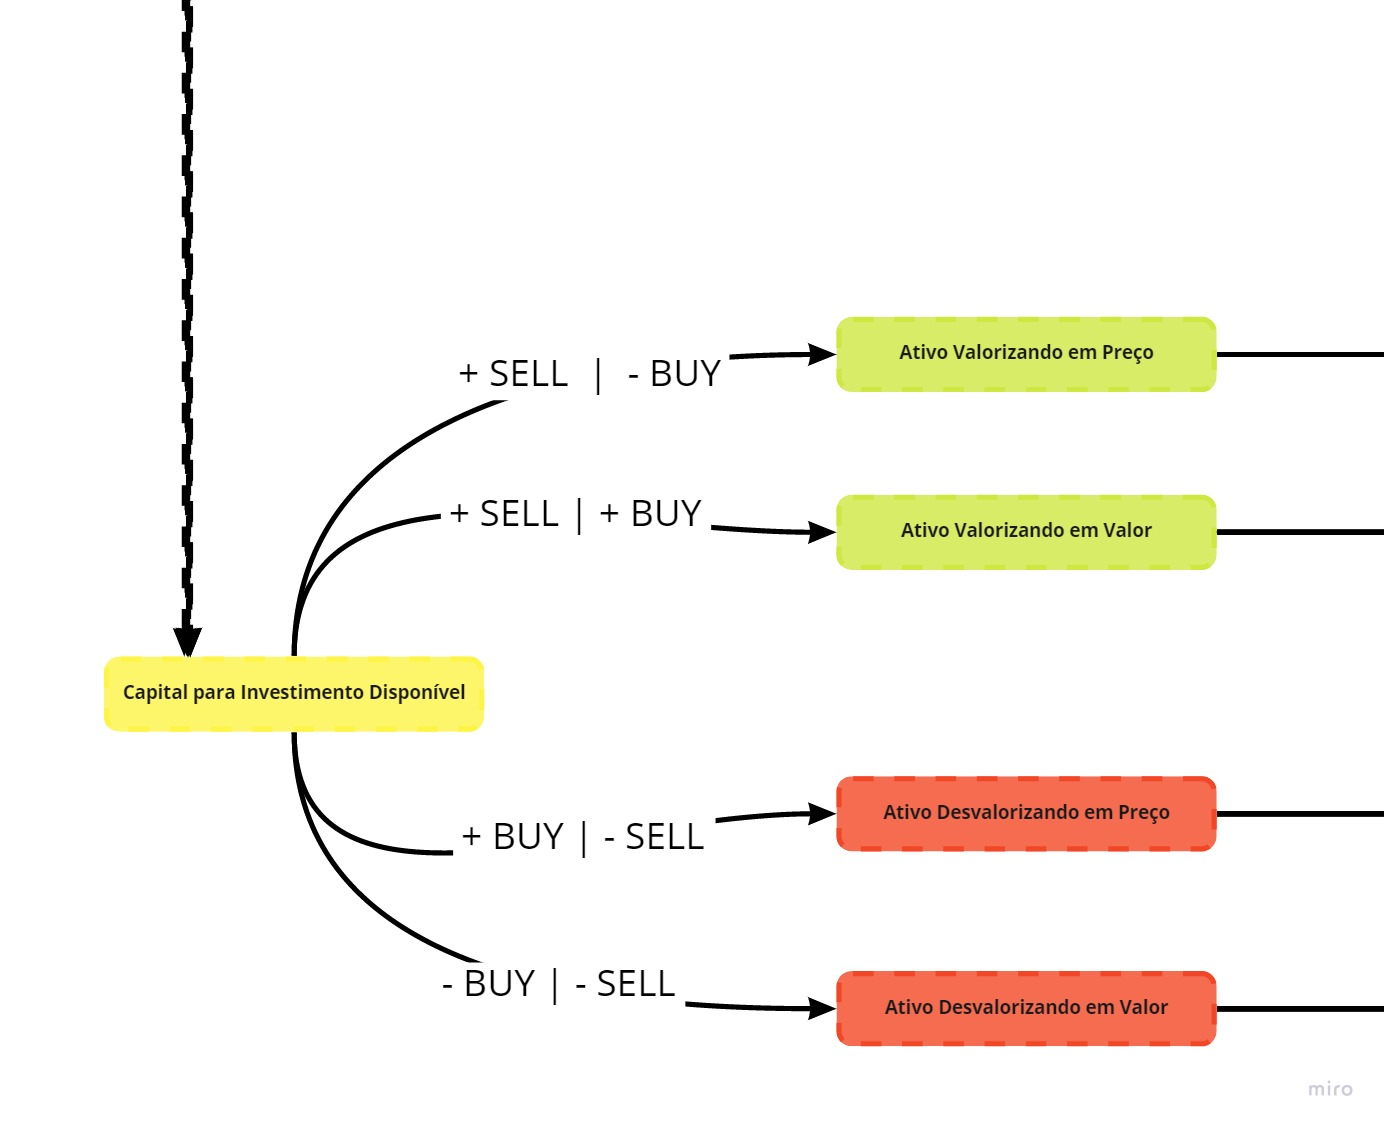
\includegraphics[width=15cm]{SIMUL/leftside.jpg}
    \caption{Grafo de Tomada de Decisão.}
    \label{fig:g1}
\end{figure}
\FloatBarrier

As chamadas apontando para cada classe indicam qual a tendência de operação sobre a classe de ativo, por exemplo, ativos com apreciação e valor são interessantes de comprar e vender, mas já os com apreciação em seu preço são interessantes de se vender e não comprá-los até haver uma mudança em seus fundamentos.

Perceba, também, que os fatores definidos indicam ações diferentes para cada classe de ativo:

\FloatBarrier
\begin{figure}[h]
    \centering
    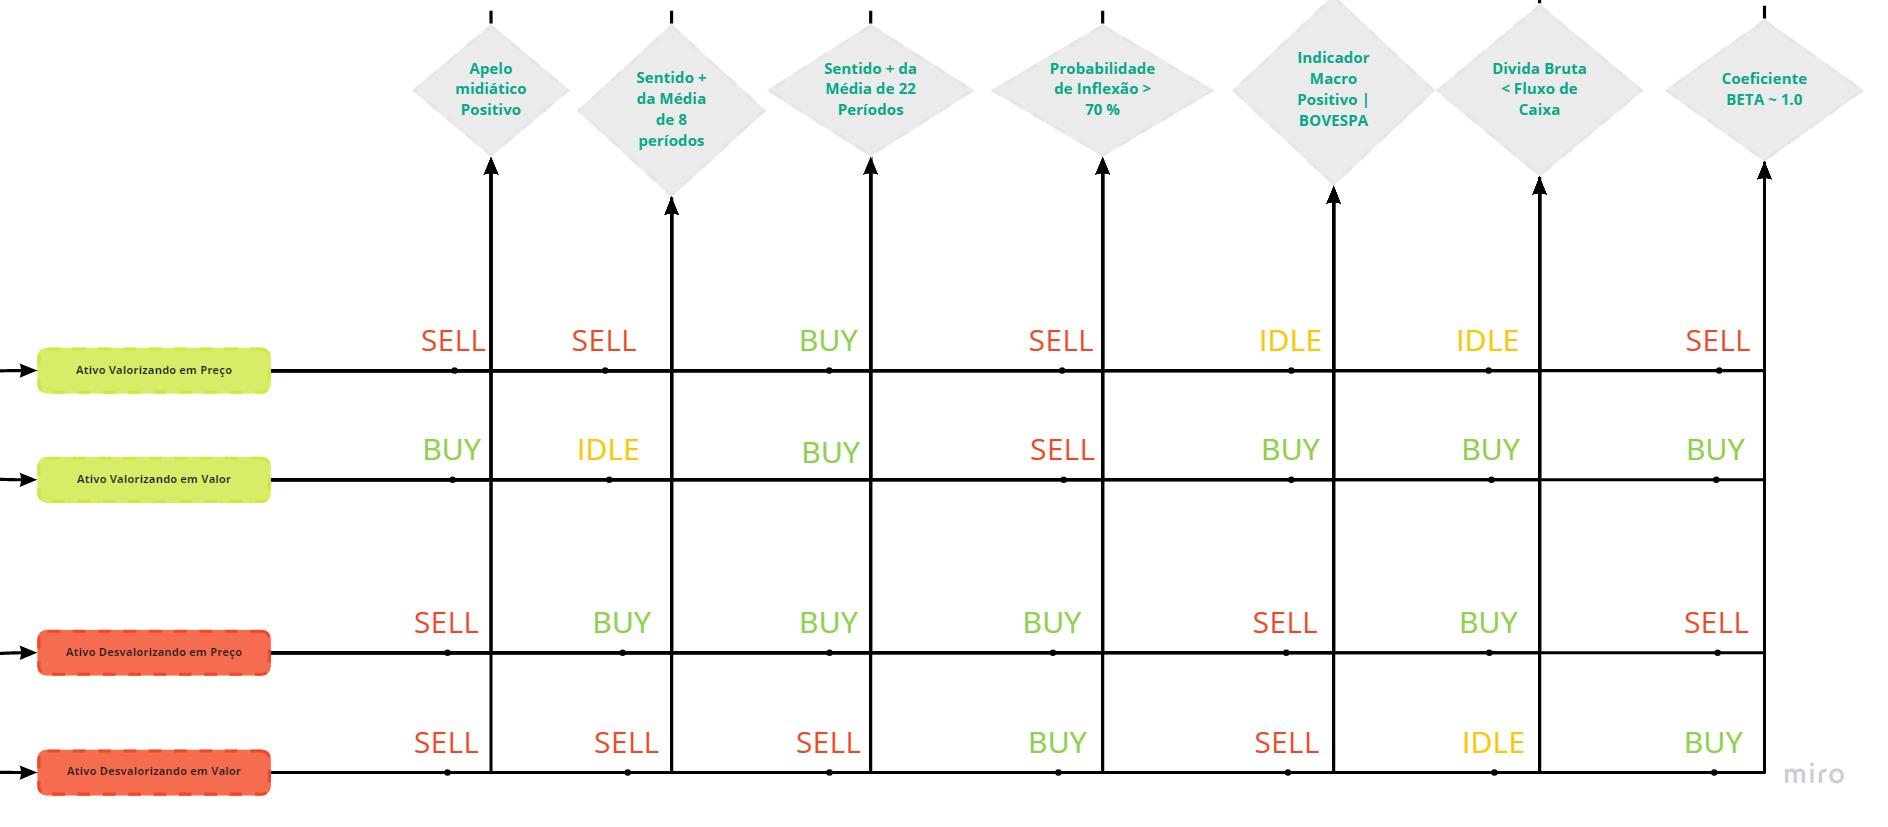
\includegraphics[width=18cm]{SIMUL/rightside.jpg}
    \caption{Grafo de Tomada de Decisão.}
    \label{fig:g1}
\end{figure}
\FloatBarrier

Consideramos importantes fatores de decisão: a pressão midiática; a tendência das médias móveis; um possível sinal de reversão ou regressão a média majoritária da tendência; a saúde do mercado no aspecto geral; o quão arriscado é o ativo em si; e se ele é rentável.

Note que utilizamos as palavras: {\it sell, buy, idle}, respectivamente, vender, comprar e não-mexer. Elas indicam para qual lado devemos tomar nossas ações, ou seja, se devemos retirar capital do investimento em dado momento, mantê-lo ou aumentar a posição.

Para cada classe de ativo, foram definidas funções com bases nas instruções mostradas na imagem acima com relação ao valor obtido para o mês. Cada instrução tem um peso definido que modifica o percentual de capital a ser alocado no fim de cada trimestre pelo investidor.

Nosso método consiste, portanto, no uso de fórmulas ponderadas para cada classe de ativo, variando no peso de suas ações em relação aos indicadores. Ao final da simulação mês a mês, é computado um valor dos pesos que indica se devemos aplicar mais capital no ativo ou se devemos remover o capital já alocado nele.



\section{Resultados}

Primeiramente, mostraremos os valores obtidos para cada indicador em cada mês.

Com relação ao apelo da mídia: 

\FloatBarrier
\begin{sidewaysfigure}[h]
    \centering
    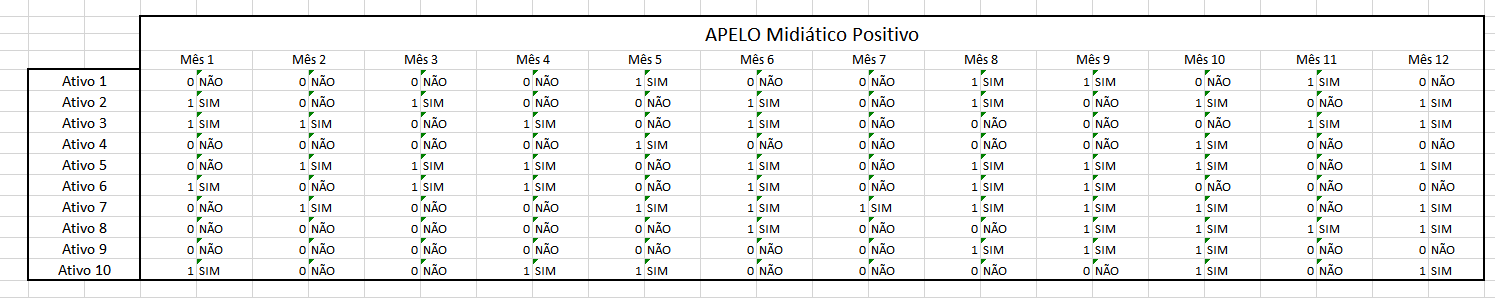
\includegraphics[width=20cm]{SIMUL/apelo.PNG}
    \caption{Apelo Midiático.}
    \label{fig:g1}
\end{sidewaysfigure}
\FloatBarrier

Com relação ao índice BOVESPA:

\FloatBarrier
\begin{sidewaysfigure}[h]
    \centering
    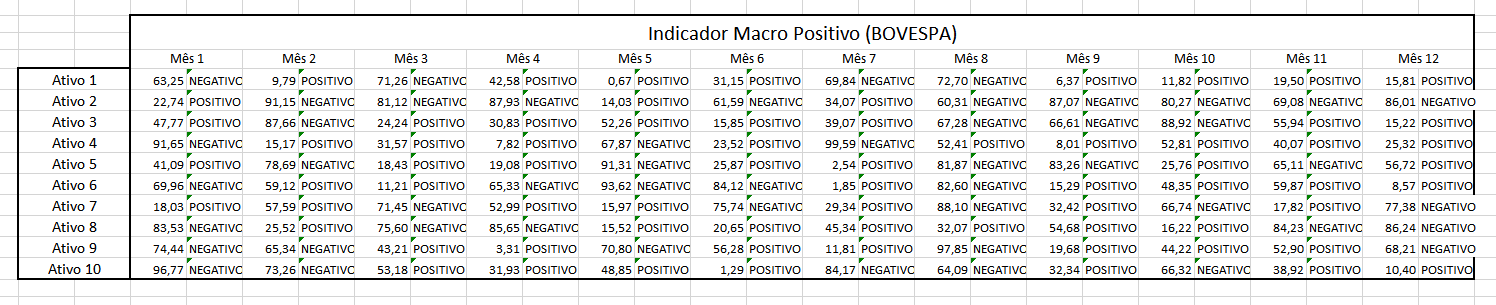
\includegraphics[width=20cm]{SIMUL/bova.PNG}
    \caption{Status de saúde para o índice BOVESPA.}
    \label{fig:g1}
\end{sidewaysfigure}
\FloatBarrier

Com relação à dívida bruta e o fluxo de caixa:

\FloatBarrier
\begin{figure}[h]
    \centering
    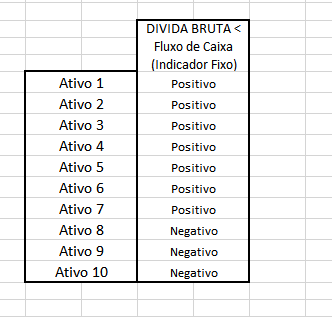
\includegraphics[width=15cm]{SIMUL/divbruta.PNG}
    \caption{Dívida bruta e o fluxo de caixa.}
    \label{fig:g1}
\end{figure}
\FloatBarrier

Com relação às médias de 8 períodos:

\FloatBarrier
\begin{sidewaysfigure}[h]
    \centering
    
\includegraphics[width=20cm]{SIMUL/m8.PNG}
    \caption{Médias de 8 períodos.}
    \label{fig:g1}
\end{sidewaysfigure}
\FloatBarrier

Com relação às médias de 22 períodos:

\FloatBarrier
\begin{sidewaysfigure}[h]
    \centering
    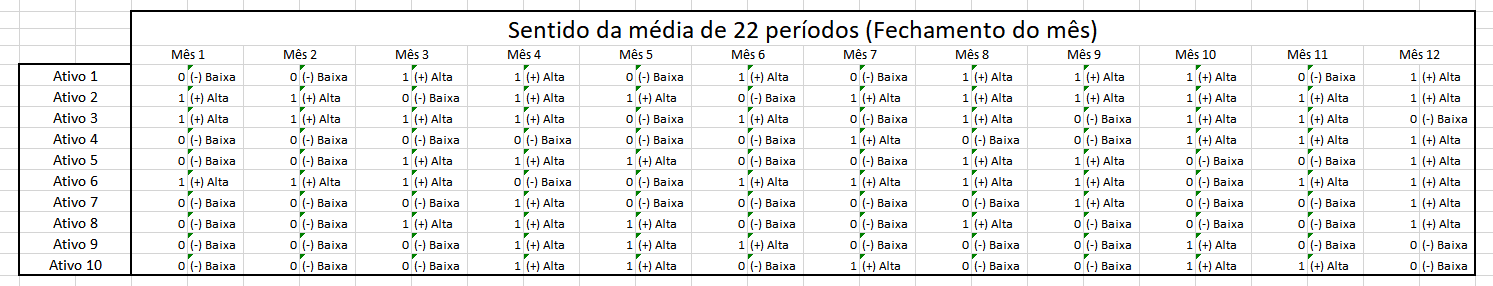
\includegraphics[width=20cm]{SIMUL/m22.PNG}
    \caption{Médias de 22 períodos.}
    \label{fig:g1}
\end{sidewaysfigure}
\FloatBarrier


Com relação às reversões de tendência:

\FloatBarrier
\begin{sidewaysfigure}[h]
    \centering
    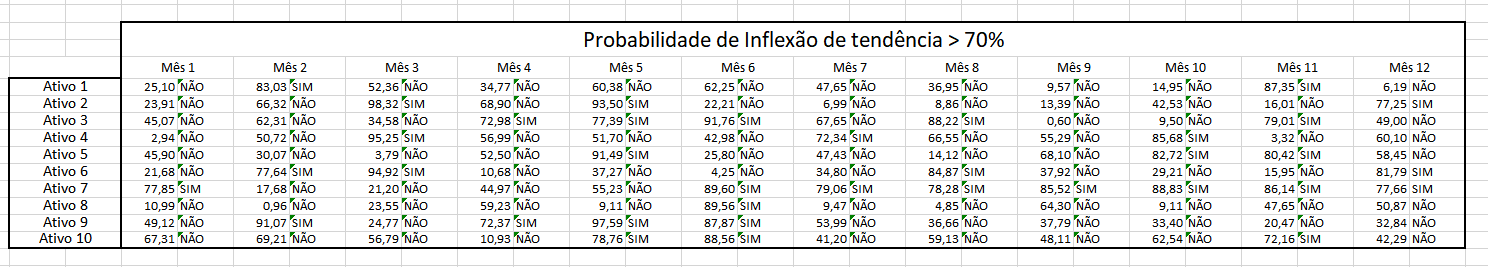
\includegraphics[width=20cm]{SIMUL/tendency.PNG}
    \caption{Reversões de tendência.}
    \label{fig:g1}
\end{sidewaysfigure}
\FloatBarrier


Depois de obter estes valores, estipulamos um coeficiente de valorização para os ativos:

\FloatBarrier
\begin{sidewaysfigure}[h]
    \centering
    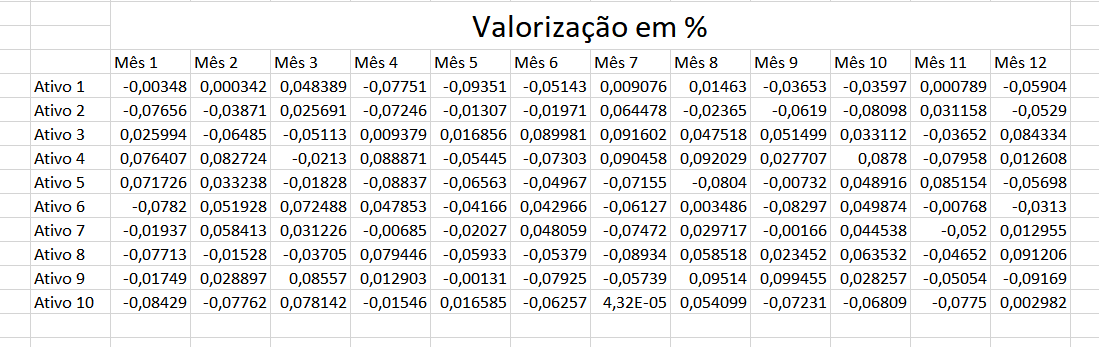
\includegraphics[width=20cm]{SIMUL/valoriza.PNG}
    \caption{Valorização.}
    \label{fig:g1}
\end{sidewaysfigure}
\FloatBarrier


Então, aplicamos estes valores nas fórmulas definidas abaixo e estimamos, para um capital de 10 milhões, em quais ativos ele estaria melhor aplicado.

\FloatBarrier
\begin{sidewaysfigure}[h]
    \centering
    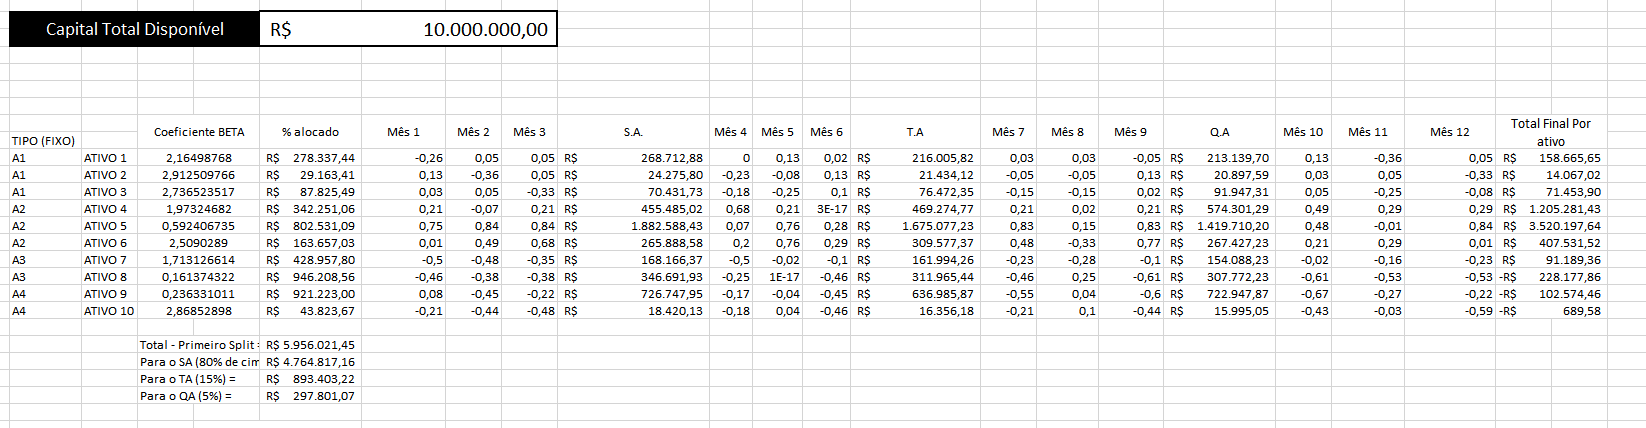
\includegraphics[width=20cm]{SIMUL/Capital_meses.PNG}
    \caption{Valorização.}
    \label{fig:g1}
\end{sidewaysfigure}
\FloatBarrier

A imagem abaixo descreve os nomes das variáveis e os pesos para cada item nas fórmulas.

\FloatBarrier
\begin{sidewaysfigure}[h]
    \centering
    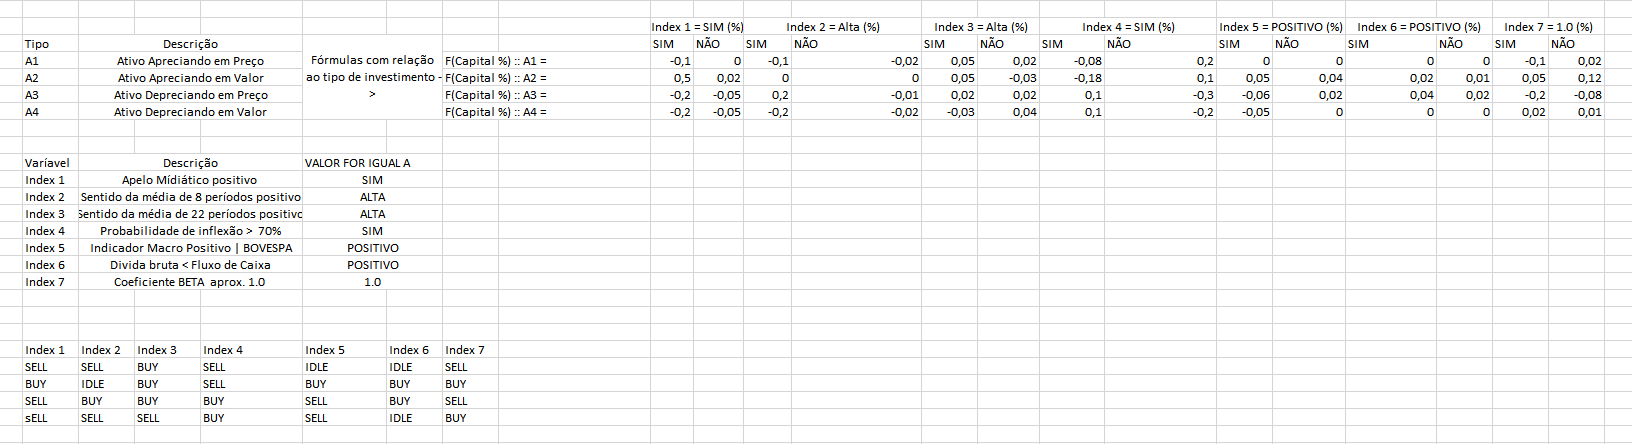
\includegraphics[width=20cm]{SIMUL/description.PNG}
    \caption{Valorização.}
    \label{fig:g1}
\end{sidewaysfigure}
\FloatBarrier

Os resultados obtidos pela equipe demonstram que as classes de ativos apreciando foram menos prejudiciais ao montante resultante, mesmo que seja possível ter momentos oportunos com ativos em desvalorização. Observa-se que, ao final de cada trimestre o impacto se agravou mais e mais, e não houve uma melhora para os maus investimentos feitos. Em compensação, os juros compostos fizeram diferença no fim para ativos A1 e A2, porém apenas os A2 tiveram lucro por manter o foco em comprar mais em vez de tentarem aproveitar momentos de mercado como os A1.


\section{Considerações Finais}

Os resultados obtidos apontam que a classe de ativos classe A2 (ativos apreciando em seu valor) obtiveram uma valorizaram do montante aplicado no período analisado, enquanto, até ativos com apreciação mas sem fundamentos não renderam junto aos ativos que depreciaram. Houve perdas expressivas nos ativos de classe A3 e A4, o que demonstra que mesmo a especulação destes não ajuda a recuperar o patrimônio mal-alocado. Porém, há de se pensar que é fácil valorizar o montante em ativos apreciando em seu preço somente, e este detalhe surtiu adversos aos esperados pela equipe: mesmo com os índices apontando alta, a falta de bons momentos de entrada e desvalorizações periódicas desta classe fizeram com que muito do capital alocado tivesse sido mal-investido.

Portanto, a equipe reconhece que a forma de valorizar o patrimônio de investidores se dá nos investimentos em ativos com apreciação em seu valor e bons fundamentos, e que não se deve entrar em ativos que estão sendo falados positivamente, ainda que sejam bons ativos, devido a reversões de tendência e ciclos de mercado.


\printbibliography  \iffalse Mostra as referências em mybib.bib. \fi

\end{document}
